%!TEX program = lualatex
\documentclass[border=0mm,11pt]{standalone}
%\usepackage{color}
%\usepackage{tikz}
\usepackage[T1]{fontenc}
\usepackage[sc]{mathpazo}
\usepackage{tikz-feynman}
\usepackage{amsmath}
\tikzfeynmanset{compat=1.1.0}


\begin{document}

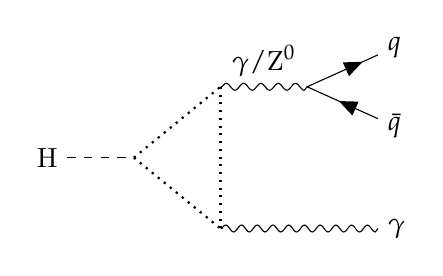
\begin{tikzpicture}[]
    \begin{feynman}
    \vertex (h) {H};
    \vertex [right=of h, xshift=-0.4cm, yshift=-0.0cm] (cent);
    \vertex [right=of cent, xshift=-0.4cm, yshift=0.9cm] (b);
    \vertex [right=of b, xshift=-0.4cm, yshift=-0.0cm] (a);
    \vertex [right=of cent, xshift=-0.4cm, yshift=-0.9cm] (d);
    \vertex [right=of d, xshift=0.5cm, yshift=-0.0cm] (c) {$\gamma$};
    \vertex [right=of b, xshift=0.5cm, yshift=0.5cm] (s1) {$q$};
    \vertex [right=of b, xshift=0.5cm, yshift=-0.5cm] (s2) {$\bar{q}$};

    \diagram* {
    (h) -- [scalar] (cent),
    (cent) -- [ghost] (b) -- [boson, edge label=\(\gamma/\text{Z}^{0}\)] (a),
    (cent) -- [ghost] (d) -- [boson] (c),
    (b) -- [ghost] (d),
    (s1) -- [with reversed arrow=0.45] (a) -- [with reversed arrow=0.68] (s2),
    };
    \end{feynman}
\end{tikzpicture}

\end{document}